\documentclass[11pt,a4paper]{article}

\usepackage{../../templates/style}

\begin{document}

\begin{problem}{กรอบสี (frame)}{standard input}{standard output}{1 second}{16 megabytes}

บนระนาบสองมิติมีกรอบสี่เหลี่ยมหลากสีวางอยู่ เอาแผ่นกระดาษสี่เหลี่ยมอีกหนึ่งแผ่นวางลงไป ต้องการทราบว่ากระดาษนั้น ทับกับพื้นที่ภายในกรอบสี่เหลี่ยมทั้ง หมดกี่กรอบ การระบุตำแหน่งของกรอบสี่เหลี่ยมและกระดาษทำโดยระบุพิกัดของจุดมุมบนซ้ายและจุดมุมล่างขวา กระดาษจะทับกับกรอบสี่เหลี่ยมถ้าพื้นที่ในระนาบร่วมระหว่างพื้นที่ในกรอบกับกระดาษมีมากกว่า $0$ (นั่นคือถ้าพบกันที่จุดมุมหรือแค่ที่ขอบจะไม่ถือว่าเป็นการทับกัน)

                ยกตัวอย่างเช่น ถ้ามีกรอบสี่เหลี่ยม $3$ กรอบดังรูปด้านล่างซ้าย สี่เหลี่ยมทั้ง สามสามารถระบุตำแหน่งได้เป็น $(1,8)$ - $(5,1)$, $(2,6)$ - $(9,2)$ และ $(6,7)$ - $(9,3)$ ถ้ามีวางกระดาษลงไปยังตำแหน่ง $(0,3)$ - $(6,0)$ หรือที่ตำแหน่ง $(2,9)$ - $(7,6)$ จะทับกับกรอบสี่เหลี่ยม $2$ รูป ถ้าวางกระดาษที่ตำแหน่ง $(3,5)$ - $(8,4)$ จะทับกับกรอบสี่เหลี่ยม $3$ รูป

         
                
\begin{figure}[h!]
\centering
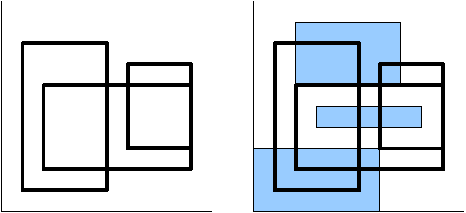
\includegraphics[width=0.7\textwidth]{../latex/img/1065/1065-1.png}
\end{figure}


  แม้ว่าจะมีกระดาษวางลงไปหลายแผ่น ให้พิจารณาว่าการวางกระดาษแต่ละแผ่นไม่เกี่ยวข้องกัน
  
\bigskip
\underline{\textbf{โจทย์}}  เขียนโปรแกรมรับข้อมูลตำแหน่งของกรอบสี่เหลี่ยม จากนั้น รับตำแหน่งของกระดาษที่วางลงไปแต่ละแผ่น แล้วคำนวณว่ากระดาษแต่ละแผ่นนั้น ทับกับกรอบสี่เหลี่ยมกี่กรอบ

\InputFile

\textbf{บรรทัดแรก} ระบุจำนวนเต็มสองจำนวน $N$ และ $M$ $(1 \leq N \leq 1\,000; 1 \leq M \leq 1\,000)$

\textbf{บรรทัดที่ $2$ ถึง $N+1$} ระบุตำแหน่งของกรอบสี่เหลี่ยมแต่ละกรอบ กล่าวคือในบรรทัดที่ $i+1$ สำหรับ $1 \leq i \leq N$ จะระบุจำนวนเต็มสี่จำนวน $X1_i$ $Y1_i$ $X2_i$ $Y2_i$ (แต่ละจำนวนมีค่าระหว่าง $-30\,000$ ถึง $30\,000;$ $X1_i < X2_i ; Y1_i > Y2_i$) เพื่อระบุว่ากรอบสี่เหลี่ยมที่ $i$ มีจุดมุมบนซ้ายที่ตำแหน่ง $(X1_i, Y1_i)$ จุดมุมล่างขวาที่ตำแหน่ง $(X2_i, Y2_i)$

\newpage
\textbf{บรรทัดที่ $N+2$ ถึง $N+M+1$} ระบุข้อมูลของกระดาษแต่ละแผนที่วางลงไป กล่าวคือ ในบรรทัดที่ $N + j+1$ สำหรับ $1 \leq j \leq M$ จะระบุจำนวนเต็มสี่จำนวน $A1_j$ $B1_j$ $A2_j$ $B2_j$ (แต่ละจำนวนมีค่าระหว่าง $-30\,000$ ถึง $30\,000; A1_j < A2_j ; B1_j > B2_j)$ เพื่อระบุว่ากระดาษแผ่นที่ $j$ เมื่อวางลงในระนาบแล้ว มีจุดมุมบนซ้ายที่ตำแหน่ง $(A1_j, B1_j)$ จุดมุมล่างขวาที่ตำแหน่ง $(A2_j, B2_j)$

\OutputFile

\textbf{มี $M$ บรรทัด} บรรทัดที่ $j$ สำหรับ $1 \leq j \leq M$ ระบุจำนวนกรอบสี่เหลี่ยมที่ทับกับกระดาษแผ่นที่ $j$

\Examples

\begin{example}
\exmp{3 3
1 8 5 1
2 6 9 2
6 7 9 3
0 3 6 0
2 9 7 6
3 5 8 4}{2
2
3}%
\end{example}

\Source

การแข่งขัน YTOPC กุมภาพันธ์ 2552

\end{problem}

\end{document}